\section{Klassische Enterprise-Architektur}

%%%%%%%%%%%%%%%%%%%%%%%%%% Monolith Architecture %%%%%%%%%%%%%%%%%%%%%%%%%%%

\begin{frame}{Monolith Architecture}
    \begin{itemize}
        \item Monolith ist altgriechisch für \textit{einheitlicher Stein}
        \item Einheitlich: Alles ist eins - alle Funktionalitäten in einer Komponente
        \item Stein: Altes Material - früher gut. Heute schlecht?
        \item Problem: Enge Kopplung
    \end{itemize}
\end{frame}

\begin{frame}{Monolith Architecture: Beispiel E-Commerce}
    \begin{figure}[!h]
        \centering
        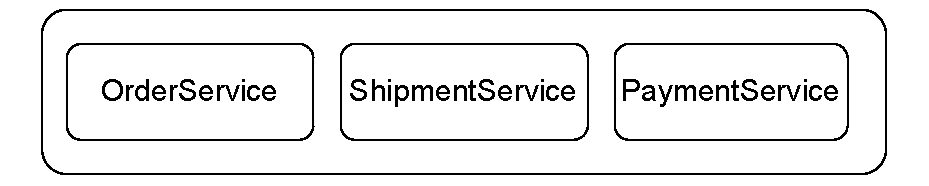
\includegraphics[scale=0.70]{imglib/mono/mono}
        \caption{E-Commerce-Beispiel mit Monolith Architektur}
        \label{fig:mono-ecommerce}
    \end{figure}
\end{frame}

\begin{frame}{Monotlith Architecture: Agilität}
    \begin{itemize}
        \item Enge Kopplung ist fatal
        \begin{itemize}
            \item Keine kleinen autonomen Teams
            \item Erhöhte Komplexität und schwere Wartung $\Rightarrow$ längere Iterationen $\Rightarrow$ unflexibel
            \item Funktionalitäten nicht wiederverwendbar $\Rightarrow$ Mehraufwand \& Duplikation $\Rightarrow$ Änderungen teuer
            \item Isolierte Funktionstests sind möglicherweise aufwendig
        \end{itemize}
        \item Auslieferung nur im Ganzen \& längere Iterationen $\Rightarrow$ seltene Auslieferung
        \item Horizontale Skalierung kaum möglich
        \item Aber: System ist nicht verteilt $\Rightarrow$ Keine Intersystemkommunikation $\Rightarrow$ Geringe Time-to-Market \& möglicherweise einfache System-Tests
        \item Ideal für lokale Anwendungen ohne Skalierungsbedarf bei welchen Flexibilität nicht notwendig ist
    \end{itemize}
\end{frame}

%%%%%%%%%%%%%%%%%%%%%%%%%% Modular Monolith Architecture %%%%%%%%%%%%%%%%%%%%%%%%%%%

\begin{frame}{Modular Monolith Architecture}
    \begin{itemize}
       \item Bisher: Eng gekoppelte Komponenten mit gegenseitigen Abhängigkeiten
       \item Jetzt: Module minimal gekoppelt und durch klare Schnittstellen definiert
       \item Alternative zur monolithischen Architektur, um die Abhängigkeiten zu reduzieren
       \item Abhängigkeiten bestehen weiterhin, müssen jedoch vom Entwickler auf ein Minimum reduziert werden
     \end{itemize}
\end{frame}

\begin{frame}{Monolith Architecture: Beispiel E-Commerce II}
    \begin{figure}[!h]
        \centering
        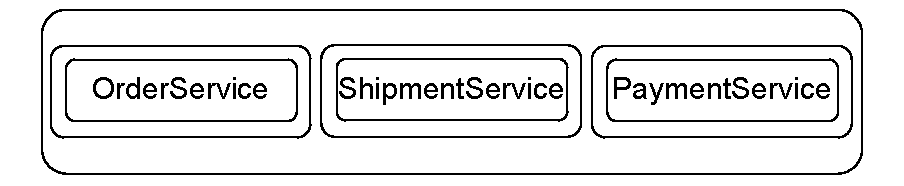
\includegraphics[scale=0.70]{imglib/mono/mono-example}
        \caption{Aufbau einer Modular monolitische Architektur}
        \label{fig:mono-modular}
    \end{figure}
\end{frame}

\begin{frame}{Modular Monolith Architecture: Agilität}
    \begin{itemize}
      \item Da Module miteinander verbunden sind, ist die Skalierung von einzelnen Modulen schwierig
      \item Abhängigkeiten zwischen Module verhindern weiterhin die parallele Entwicklung von Modulen
      \item Fehler in einem Modul können die Verfügbarkeit des gesamten System beeinträchtigen
    \end{itemize}
\end{frame}
